\documentclass[a4paper]{article}

\usepackage{xcolor}
\usepackage{fancyheadings}
\usepackage{listings}
\usepackage{graphicx}
\usepackage[utf8]{inputenc}
\usepackage{multirow}
\lstset{frameround=fttt,numbers=left,breaklines=true, extendedchars=true}

\newcommand{\todo}[1]{\textcolor{red}{[#1]}}
\lhead{Open Universiteit}
\chead{IM0202, Software evolution}
\rhead{Assignment 1}

\begin{document}
\pagestyle{fancy}

\section*{Studentgegevens}
\begin{description}
	\item [Cursuscode] IM0202
	\item [Naam] Ewoud Westerbaan
	\item [Studentnummer] 852069942
	\item [Naam] Martin de Boer
	\item [Studentnummer] 837372832
\end{description}

\section{Samenwerking}
Bij de start van het practicum zijn we parallel aan elkaar aan onze "eigen" modules begonnen: Main.rsc, Volume.rsc en Duplicates.rsc door Ewoud, en UnitSize.rsc, Complexity.rsc, Aggregate.rsc en Rate.rsc door Martin. Gaandeweg het project zijn we intensiever gaan samenwerken: Ewoud heeft Utils.rsc gemaakt waarin code is opgenomen die door meerdere modules wordt aangeroepen, en Martin heeft een opzet gemaakt voor de unittesten. Tijdens het bugfixen hebben we ook elkaars modules verder verbeterd. De diverse modules worden hieronder kort toegelicht.

\section{Structuur}
\label{sec:Structuur}
De volgende modules zijn in het Rascal project opgenomen:
\begin{description}
\item[Main.rsc] De hoofdmodule. Van hieruit worden de andere modules aangeroepen en wordt de uitvoer gegenereerd.
\item[metrics::Volume.rsc] Berekent het volume (LOC) van de SmallSQL aplicatie. Wij interpreteren het volume als alle regels code in een java file, zonder commentaar en zonder de lege ruimtes, zoals ook in \cite{A}. Hieronder beschouwen wij ook velddefinities, constantendefinities, import statements e.d.
\item[metrics::UnitSize.rsc] Berekent het aantal regels code per unit (methode / constructor). Er zijn verschillen in de som van de unitsize ten opzicht van het volume. De som van de coderegels in units is de som van de inhoud van de methodes en constructoren.
\item[metrics::Complexity.rsc] Bepaalt de complexiteit per unit. We gaan er vanuit dat de standaard complexiteitsmaat de waarde 1 heeft en dat er voor een aantal taalconstructies reden is om deze met 1 te verhogen.
\item[metrics::Duplicate.rsc] Zoekt de dubbele code in de sources van SmallSQL. Onze aanname is dat het aantal duplicate regels het totaal van regels is dat meerdere keren in de applicatie voorkomt.
\item[metrics::Aggregate.rsc] Aggregeert de gegevens van de bovenstaande modules en bepaalt de percentages t.b.v. de rating. Hierbij wordt rekening gehouden met de som van de unit sizes (en niet het totale volume, zie boven).
\item[metrics::Rate.rsc] Bepaalt de rating van SmallSQL per onderdeel (unit size, complexiteit en duplicaten).
\item[utils::Utils] Bevat een aantal utility functies.
\end{description}

\section{Betrouwbaarheid}
De betrouwbaaheid en de juistheid van de oplossing kunnen we waarborgen door het gebruik van unittests. 
We hebben meerdere `dummy'-projecten gemaakt die dienen als referentieproject bij het draaien van deze tests. 
Door dat we zelf deze projecten maken, welke klein en overzichtelijk zijn, kunnen we vrij specifiek meten, testen en de juistheid valideren van de opgeleverde code. In Listing \ref{lst:testoutput} is de output weergegeven van onze unittests.
\begin{lstlisting}[caption={Unit test output},label={lst:testoutput},frame = single]
Running tests for tests::metrics::VolumeTest
Test report for tests::metrics::VolumeTest                                                
        all 3/3 tests succeeded
Running tests for tests::metrics::AggregateTest
Test report for tests::metrics::AggregateTest                                             
        all 4/4 tests succeeded
Running tests for tests::utils::TestUtilsTest
Test failed. Msg: ** No worries! This test should fail **. Expected = 1, actual = 2       
Test failed. Msg: ** No worries! This test should fail **. Expected = blabla, actual = bla
Test report for tests::utils::TestUtilsTest                                 
        all 5/5 tests succeeded
Running tests for tests::utils::UtilsTest
Test report for tests::utils::UtilsTest                                                     
        all 18/18 tests succeeded
Running tests for tests::metrics::UnitSizeTest
Test report for tests::metrics::UnitSizeTest                                              
        all 2/2 tests succeeded
Running tests for tests::metrics::DuplicationTest
Test report for tests::metrics::DuplicationTest                                             
        all 13/13 tests succeeded
Running tests for tests::metrics::ComplexityTest
Test report for tests::metrics::ComplexityTest                                            
        all 2/2 tests succeeded
Running tests for tests::metrics::RateTest
Test report for tests::metrics::RateTest                                                    
        all 11/11 tests succeeded
\end{lstlisting}
\section{Resultaten en interpretatie}
In Listing \ref{lst:output} is de output van het geschreven programma te zien over SmallSQL. 

\begin{lstlisting}[caption={Programma output SmallSQL},label={lst:output},frame = single]
Volume berekenen ...
Berekend volume: 
- totaal aantal regels (incl. lege regels): 35271
- commentaarregels: 4102
- coderegels: 22192

Unit size berekenen ...
Aantal gevonden units (methodes en constructoren): 2494
Som van de aantallen regels per methode/constructor: 
- totaal aantal regels (incl lege regels binnen de units): 22730
- commentaarregels: 628
- coderegels: 16401

Aggregeren gegevens (unit size verhoudingen) ...
- Categorie Insane (Extremely large units (>250)): 3%
- Categorie Very large (Very large units (101-250)): 8%
- Categorie Medium (Medium size units (16-50)): 35%
- Categorie Large (Large units (51-100)): 14%
- Categorie Small (Small units (0-15)): 38%
- Rank op basis van aggregatie: --

Berekenen cyclomatische complexiteit ...

Aggregeren gegevens (unit size and complexity) ...
- Categorie Simple (Without much risk): 67%
- Categorie Moderate (With moderate risk): 10%
- Categorie Untestable (Untestable, very high risk): 7%
- Categorie Complex (Complex, with high risk): 14%
- Rank op basis van aggregatie: --

Berekenen duplicatie ...
- Aantal duplicaties: 188
- Aantal regels gedupliceerd: 1976
- Duplicatepercentage: 12.04804585%
- Rank op basis van duplicatie: -

Programma beeindigd
\end{lstlisting}
Als we de output van \ref{lst:output} nemen en deze tegen de referentie tabellen aanhouden als in \cite{A}, kunnen we een soortgelijk resultatentabel invullen. Omdat wij unittesting niet gemeten hebben, laten we deze buiten beschouwing.

Voor de interpretatie van de unitsizes zijn door \cite{A} geen strikte waardes gegeven, daarom dienen wij hier zelf een methode voor te bedenken.
Wij kiezen ervoor om de verdeling aan te houden als in \cite{B}, zodat we de uitkomst kunnen vergelijken met de gemiddelde.

Als we de verhouding in \cite{B} aannemen, komen we op een verdeling als in Tabel \ref{tbl:UnitSizeClassificatie}.

\begin{table}[h]
\caption{Unitsize classificatie}
\label{tbl:UnitSizeClassificatie}
\begin{tabular}{|l|l|}
\hline
Unitsize         & Classificatie      \\ \hline
0-15             & small units        \\
16-50            & medium sized units \\
51-100           & large units        \\
101-150          & very large units   \\
\textgreater{}250& insane             \\ \hline
\end{tabular}
\end{table}

Wij vergelijken de uitkomst van het programma met de waardes uit \cite{B}. De applicatie die onderzocht wordt kan dan visueel vergeleken worden met \cite{B} en kan dan boven (+), onder (-) of gelijk (0) scoren. Ter referentie hebben we de grafiek uit \cite{B} toegevoegd (zie Figuur \ref{fig:RefVerdeling}).
\begin{figure}[htbp]
\caption{Percentages of SLOC}
\centering
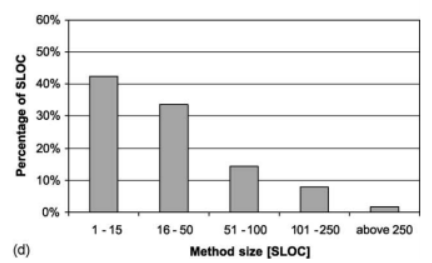
\includegraphics[width=0.6 \textwidth]{Capture.png}
\label{fig:RefVerdeling}
\end{figure}

Wel willen wij hierbij de opmerking plaatsen dat de verdeling ons inziens te grof is. Wij zijn van mening dat de verhoudingen beter kunnen. Nader onderzoek zal plaats moeten vinden om een betere verdeling te maken. Toch kiezen wij ervoor om te refereren met \cite{B}, zodat we de uitkomsten ergens aan kunnen refereren. Als we de unitsize verhoudingen vergelijken met Figuur \ref{fig:RefVerdeling}, scoort SmallSQL op het oog gelijk en krijgt daarom de waarde 0.


Als we alle waardes in de tabel zetten zoals in \cite{A}, komen we uit op Tabel \ref{tbl:ResultaatSmallSQL}. De laatste kolom hiervan lichten we toe.
\begin{description}
\item[Analysability] Analysability is afhankleijk van volume (++), complexity per unit (- - ) en unit size (0). Bij elkaar komt vinden wij dat dit een neutrale score oplevert van 0.
\item[Changeability] Omdat de complexity per unit zeer hoog is, en de hoeveelheid duplicatie ook vrij hoog is, geven we changeability de score -.
\item[Stability] We hebben de waarde van de unit testing niet gemeten. Hierdoor kunnen we niets zeggen over de stability en krijgt deze de neutrale waarde 0.
\item[Testability] Omdat we unit testing niet hebben gemeten, is de testability volledig afhankelijk van de complexity per unit. Deze is voor SmallSQL zeer hoog en daarom geven we testability de gelijke waarde als complexity per unit: - -.
\end{description}
\begin{table}[h]
\caption{Resultaat SmallSQL}
\label{tbl:ResultaatSmallSQL}
\begin{tabular}{llllllll}
                          &                                                      &                                    & \multicolumn{5}{l}{source code properties}                                                                                                                           \\ \cline{4-7}
                          &                                                      & \multicolumn{1}{l|}{}              & \multicolumn{1}{c|}{\rotatebox[origin=c]{90}{volume}} & \multicolumn{1}{c|}{\rotatebox[origin=c]{90}{ complexity per unit }} & \multicolumn{1}{c|}{\rotatebox[origin=c]{90}{duplication}} & \multicolumn{1}{c|}{\rotatebox[origin=c]{90}{unit size}} &                         \\ \cline{4-7}
                          &                                                      & \multicolumn{1}{l|}{}              & \multicolumn{1}{c|}{++}       & \multicolumn{1}{c|}{- -}                    & \multicolumn{1}{c|}{-}            & \multicolumn{1}{l|}{0}          &                         \\ \cline{3-8} 
\multirow{4}{*}{\rotatebox[origin=c]{90}{ISO 9128}} & \multicolumn{1}{l|}{\multirow{4}{*}{\rotatebox[origin=c]{90}{maintainablity}}} & \multicolumn{1}{l|}{analysability} & \multicolumn{1}{c|}{X}      & \multicolumn{1}{l|}{}                    & \multicolumn{1}{c|}{X}           & \multicolumn{1}{c|}{X}         & \multicolumn{1}{c|}{0} \\ \cline{3-8} 
                          & \multicolumn{1}{l|}{}                                & \multicolumn{1}{l|}{changeability} & \multicolumn{1}{l|}{}       & \multicolumn{1}{c|}{X}                   & \multicolumn{1}{c|}{X}           & \multicolumn{1}{l|}{}          & \multicolumn{1}{c|}{- -} \\ \cline{3-8} 
                          & \multicolumn{1}{l|}{}                                & \multicolumn{1}{l|}{stability}     & \multicolumn{1}{l|}{}       & \multicolumn{1}{c|}{}                    & \multicolumn{1}{l|}{}            & \multicolumn{1}{l|}{}          & \multicolumn{1}{c|}{0} \\ \cline{3-8} 
                          & \multicolumn{1}{l|}{}                                & \multicolumn{1}{l|}{testability}   & \multicolumn{1}{l|}{}       & \multicolumn{1}{c|}{X}                   & \multicolumn{1}{l|}{}            & \multicolumn{1}{l|}{}          & \multicolumn{1}{c|}{- -} \\ \cline{3-8} 
\end{tabular}
\end{table}

\bibliographystyle{abbrv}
\bibliography{verslag_assignment1}

\end{document}
